
\subsubsection{15.10.14}

\begin{enumerate}
	\item Время начала и окончания собрания:\newline
	17:00 - 21:30
	\item Цели собрания:\newline
	\begin{enumerate}
	  \item Заменить перекладины на подъемнике на более прочные.\newline
	  
	  \item Скрепить попарно направляющие в подъемнике для того, чтобы он ровно раздвигался.\newline
	  
    \end{enumerate}
    
	\item Проделанная работа:\newline
	\begin{enumerate}
	  \item У нас не было возможности приобрести необходимые ресурсы для доработки подъемника, поэтому сегодня было решено заняться разработкой захвата для мячей в виде вращающейся щетки.\newline
      
      \item  Передняя часть робота была видоизменена и на ней были поставлены сервопривод свободного вращения с осью, на которой было решено закрепить щетку, в качестве ворсинок которой будут использоваться стяжки.\newline
      
     \begin{figure}[H]
     	\begin{minipage}[h]{1\linewidth}
     		\center{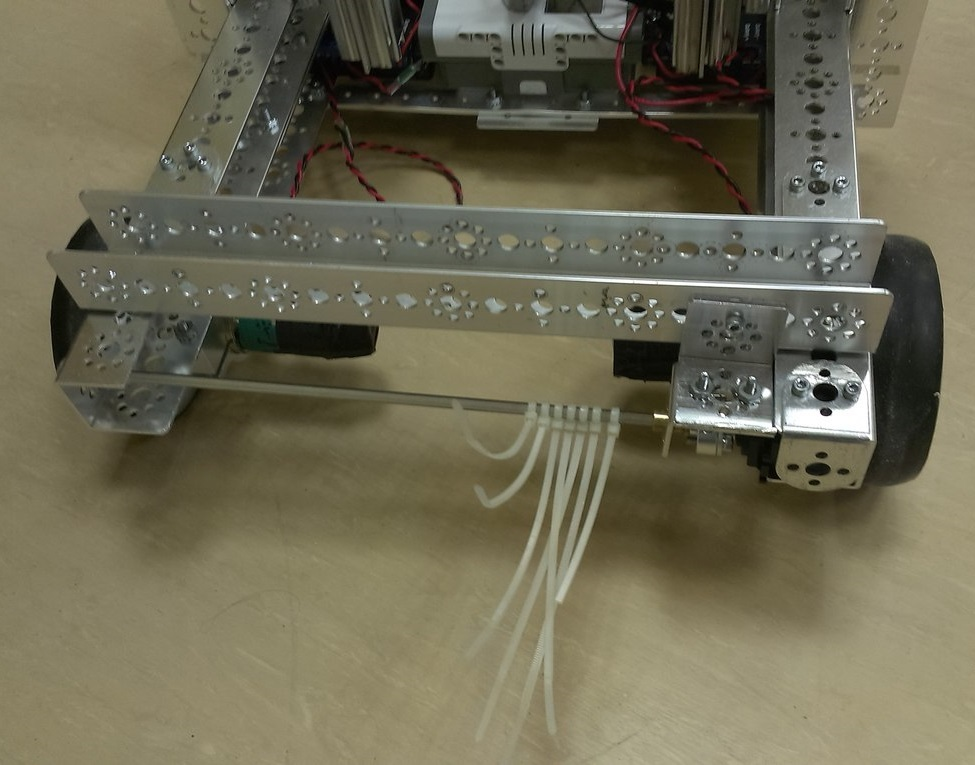
\includegraphics[height=0.9\measurepage]{days/15.10.14/images/01}}
     		\caption{Механизм захвата}
     	\end{minipage}
     \end{figure}
      
    \end{enumerate}
    
	\item Итоги собрания: \newline
	\begin{enumerate}
	  \item Создана основа захвата для мячей.\newline
	  
      \item Доработка подъемника не осуществлена.\newline
      
    \end{enumerate}
    
	\item Задачи для последующих собраний:\newline
	\begin{enumerate}
	  \item Купить все необходимые ресурсы для доработки подъемника.\newline
	  
	  \item Доделать захват для мячей и написать программу для управления им.\newline

    \end{enumerate}     
\end{enumerate}

\fillpage
